% $Header: /cvsroot/latex-beamer/latex-beamer/solutions/generic-talks/generic-ornate-15min-45min.en.tex,v 1.5 2007/01/28 20:48:23 tantau Exp $

\documentclass[xcolor=dvipsnames]{beamer}

\def\argmax{\qopname\relax{no}{argmax}}
\def\slidehead#1{\begin{frame}{#1}}
\def\cemph#1{\textcolor{blue}{#1}}
\def\bcemph#1{\textcolor{blue}{\textbf{#1}}}
\long\def\refcite#1{{\small $[$#1$]$}}

% Copyright 2004 by Till Tantau <tantau@users.sourceforge.net>.
%
% In principle, this file can be redistributed and/or modified under
% the terms of the GNU Public License, version 2.
%
% However, this file is supposed to be a template to be modified
% for your own needs. For this reason, if you use this file as a
% template and not specifically distribute it as part of a another
% package/program, I grant the extra permission to freely copy and
% modify this file as you see fit and even to delete this copyright
% notice. 


\mode<presentation>
{
  \usetheme{Warsaw}
  \usecolortheme[named=Blue]{structure}
  %\usecolortheme[named=BrickRed]{structure}

  \setbeamertemplate{blocks}[rounded][shadow=true]
  \setbeamertemplate{navigation symbols}{} 

  \setbeamercovered{transparent}
}


%% Insert slide numbers with specific foreground and background colors...
\setbeamercolor{mycolor}{fg=white,bg=black}
\defbeamertemplate*{footline}{shadow theme}{%
  \leavevmode%
  \hbox{\begin{beamercolorbox}[wd=.5\paperwidth,ht=2.5ex,dp=1.125ex,leftskip=.3cm
      plus1fil,rightskip=.3cm]{author in head/foot}%
      \usebeamerfont{author in head/foot}\hfill\insertshortauthor
    \end{beamercolorbox}%
    \begin{beamercolorbox}[wd=.4\paperwidth,ht=2.5ex,dp=1.125ex,leftskip=.3cm,rightskip=.3cm
      plus1fil]{title in head/foot}%
      \usebeamerfont{title in head/foot}\insertshorttitle\hfill%
    \end{beamercolorbox}%
    \begin{beamercolorbox}[wd=.1\paperwidth,ht=2.5ex,dp=1.125ex,leftskip=.3cm,rightskip=.3cm
      plus1fil]{mycolor}%
      \hfill\insertframenumber\,/\,\inserttotalframenumber
    \end{beamercolorbox}}%
  \vskip0pt%
}

\usepackage[english]{babel} % or whatever
\usepackage[latin1]{inputenc} % or whatever
\usepackage{listings}
\usepackage{times}
%\usepackage[T1]{fontenc}
\usepackage{amssymb}
\usepackage{amstext}
\usepackage{amsmath}

\usepackage{graphicx}
\usepackage{graphics}
\usepackage{mathptmx}
\usepackage{url}
\usepackage{subfigure}
%\usepackage{algorithm}
%\usepackage{algorithmic}
\usepackage{caption}
\usepackage{hyperref}

% mathematical notation
\def\no{\; {not} \;}
\def\myif{\texttt{:-}}
\newcommand{\defeq}{:=}
\newcommand{\stt}[1]{{\small\texttt{#1}}}
\newcommand {\oor} {\,\hbox{\it or}\;}
\newcommand{\pair}[2]{\ensuremath{(#1, #2)}}
\newcommand{\union}{\ensuremath{\cup}}
\newcommand{\rif}{\stackrel{\,\,+}{\leftarrow}}

% theorem environments
\newtheorem{property}[theorem]{}
\usefonttheme{serif}
\usefonttheme{professionalfonts}

% slide package options
\usetheme{Warsaw}

% document information

\title{Representing and Reasoning with Intentional Actions on a Robot\\
  \small{PlanRob - Architectures and Frameworks\\ICAPS 2018}} \author[Rocio Gomez] % (optional, use only with lots of authors)
{Rocio Gomez, Mohan Sridharan and Heather Riley}
% - Use the \inst{?} command only if the authors have different
%   affiliation.

\institute[The University of Auckland] % (optional, but mostly needed)
{
  %\inst{1}%
  Department of Electrical and Computer Engineering\\
  The University of Auckland, NZ 
}
\institute[University of Birmingham]
{
  %\inst{2}%
  School of Computer Science\\
  University of Birmingham, UK 
}

\date[June 2017] % (optional)
{\small{June 26, 2018}}


%%%%%%%%%%%%%%%%%%%%%%%%%%%%%%%%%%%%%%%%%%%%%%%%%%%%%%%%%%%%%%%%%%%%%%%%%%%%%%%%
%%%%%%%%%%%%%%%%%%%%%%%%%%%%%%%%%%%%%%%%%%%%%%%%%%%%%%%%%%%%%%%%%%%%%%%%%%%%%%%%

\begin{document}

\begin{frame}
    \titlepage
\end{frame}


\begin{frame}{Talk Outline}
  \begin{itemize}
    \onslide<1>
  \item  Motivation and architecture overview.
    \ \\
    \ \\
    \ \\
    \onslide<0>
  \item Knowledge representation and reasoning.
    \ \\
    \ \\
    \ \\
  \item Adapted Theory of Intentions.
    \ \\
    \ \\
    \ \\
  \item Experiments and conclusions.
  \end{itemize}
\end{frame}




%%%%%%%%%%%%%%%%%%%%%%%%%%%%%%%%%%%%%%%%%%%%%%%%%%%%%%%%%%%%%%%%%%%%%%%%%%%%%%%%
%%%%%%%%%%%%%%%%%%%%%%%%%%%%%%%%%%%%%%%%%%%%%%%%%%%%%%%%%%%%%%%%%%%%%%%%%%%%%%%%

\section{Motivation and Architecture Overview}

%%%%%%%%%%%%%%%%%%%%%%%%%%%%%%%%%%%%%%%%%%%%%%%%%%%%%%%%%%%%%%%%%%%%%%%%%%%%%%%%
\subsection{Architecture overview}

\begin{frame}\frametitle{Architecture Overview} 
  \textbf{Design architecture for robots that:}
  \begin{itemize}
  \item Use \textcolor{red}{qualitative} and
    \textcolor{red}{quantitative} descriptions of incomplete knowledge
    to improve quality and efficiency of decision making.\\
    \textcolor{blue}{``books are usually in
the library''}\\
    \textcolor{blue}{``I am $90\%$ certain the book is on the
      table''}

    \ \\
   \item Work in complex dynamic domain where unexpected things happen.

    \ \\
    \item Receive more sensor data than it can handle at reasoning level. 

 % \item Always reasoning about observations related to the \textcolor{red}{uderlying intention} enabaling it to persue this intention in dynamics domains.\\
  %  \textcolor{blue}{``Mi intention is to put all books in the libary. Can my current plan still achieve so?''}
  %\item Reasons with \textcolor{red}{tightly-coupled} transition diagrams at two different levels of abstraction.  
  \end{itemize}
\end{frame}



%%%%%%%%%%%%%%%%%%%%%%%%%%%%%%%%%%%%%%%%%%%%%%%%%%%%%%%%%%%%%%%%%%%%%%%%%%%%%%%%
\subsection{Basic Idea and Domain}

\begin{frame}\frametitle{Architecture Overview}
  \begin{figure}
    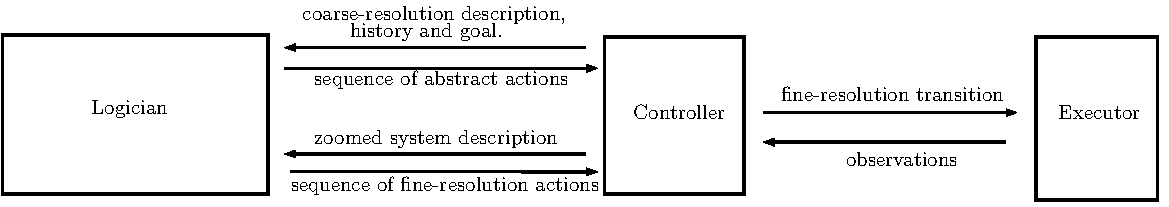
\includegraphics[width=0.8\textwidth]{Images/architecture}
  \end{figure}

\end{frame}


\begin{frame}\frametitle{Architecture Overview}
  \begin{itemize}
  \item Combine strengths of declarative programming and probabilistic
    models.
    
    \ \\
  \item \textcolor{red}{Formal relationship} between transition
    diagrams. \textcolor{blue}{Tight coupling, not a ``switch''}.

    \ \\
  \item Support \textcolor{red}{non-monotonic logic} and
    \textcolor{red}{probabilistic} representations of
    \textcolor{red}{incomplete domain knowledge} and
    \textcolor{red}{uncertainty}.

    \ \\
  \item \textcolor{red}{Interactive} and cumulative
    \textcolor{red}{relational learning}; classical and reinforcement,
    procedural and knowledge-based.

    \ \\
  \item Implemented on \textcolor{red}{robots} interacting with
    dynamic environmetns, and in \textcolor{red}{simulation}.
  \end{itemize}
\end{frame}


\begin{frame}
  \frametitle{Illustrative Domain: Robot Moving Objects}
  \begin{center}
    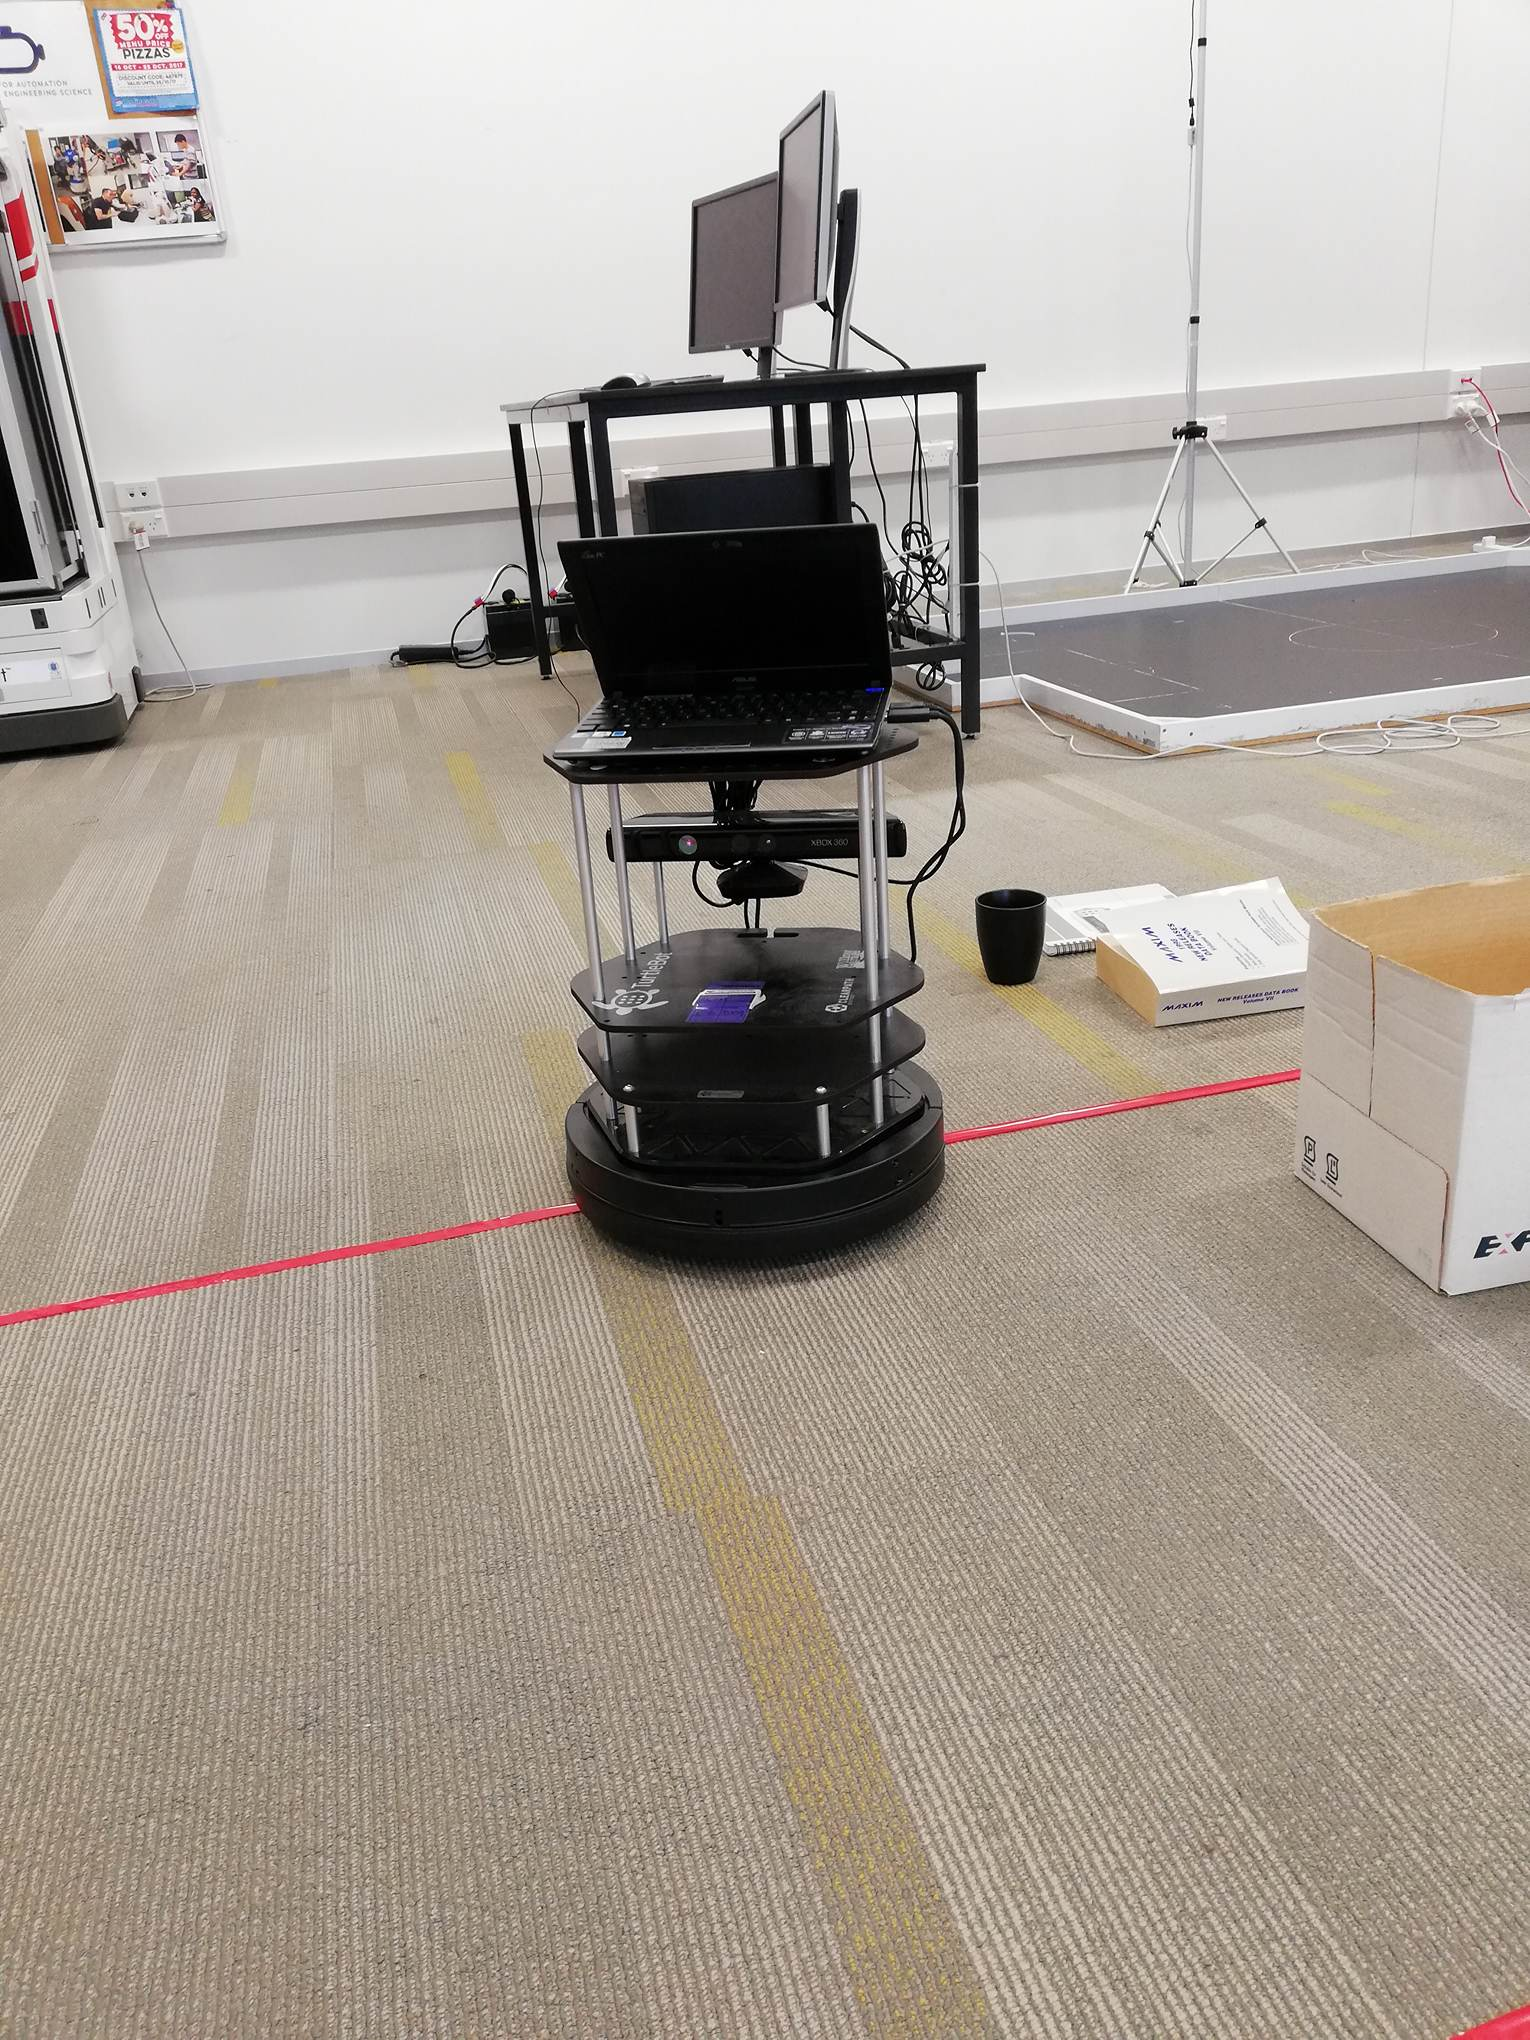
\includegraphics[height=8em]{Images/turtlebot1} \hspace{2em}
   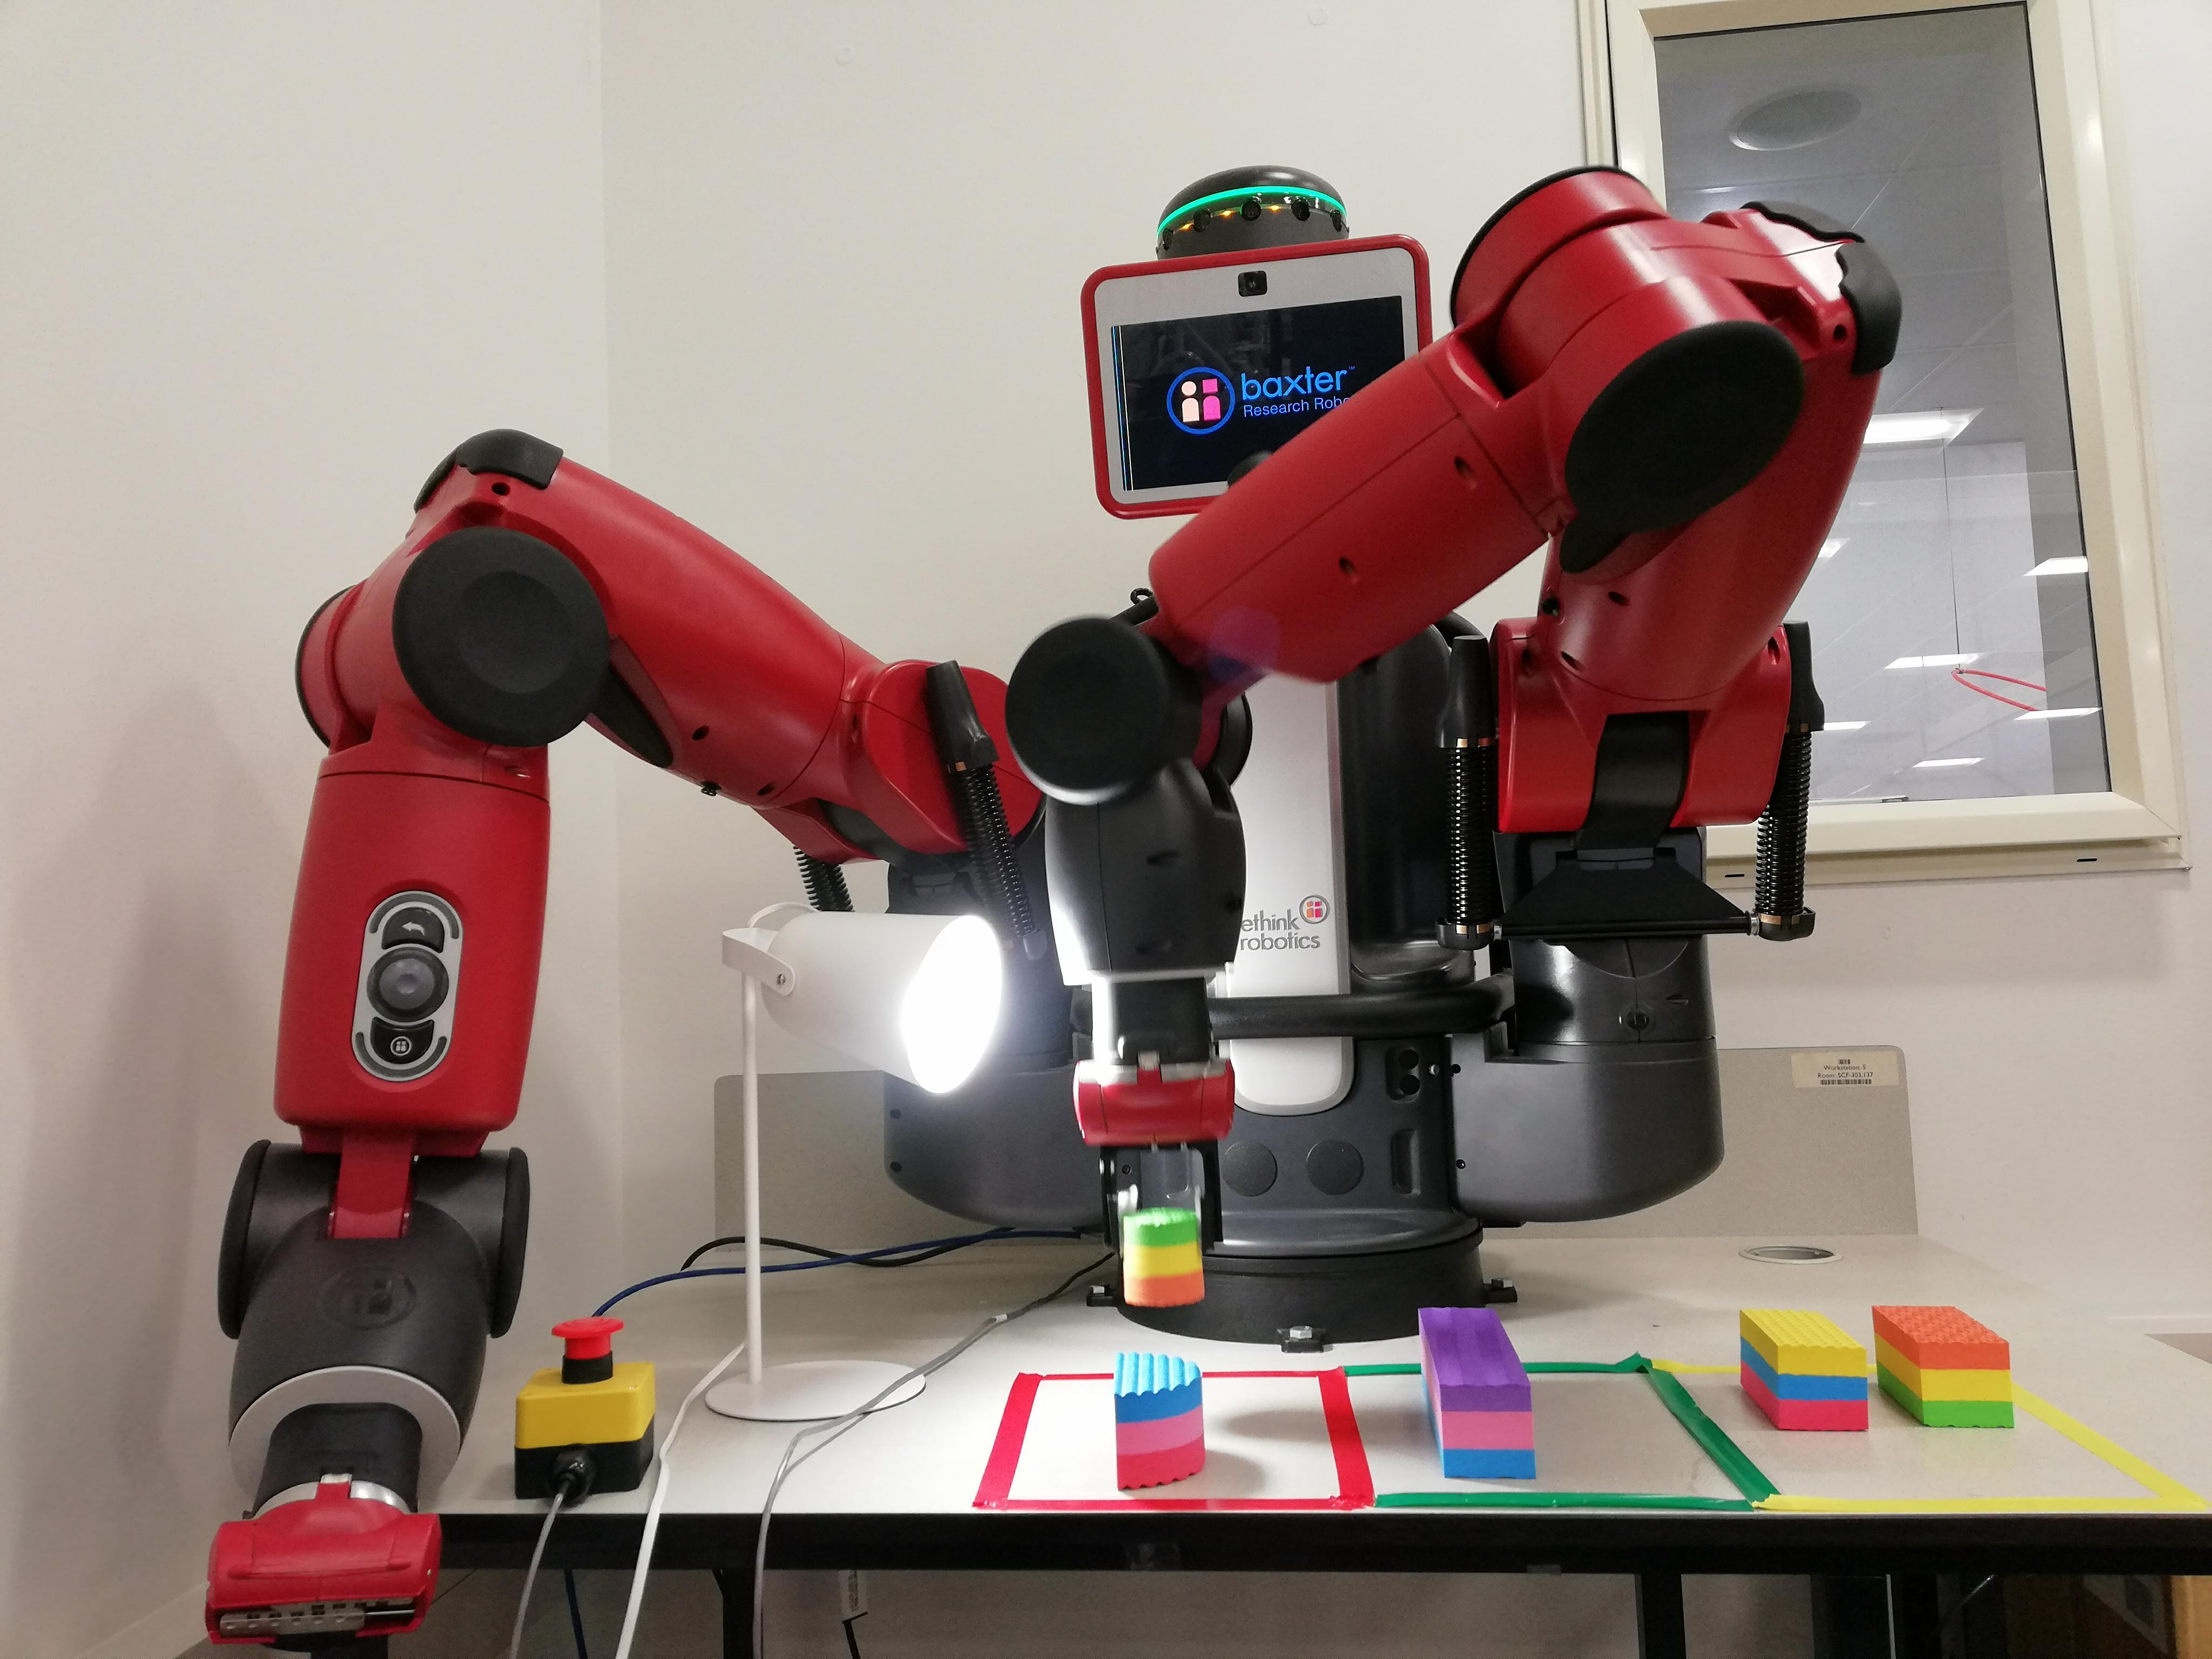
\includegraphics[height=8em]{Images/baxter1}\\
%    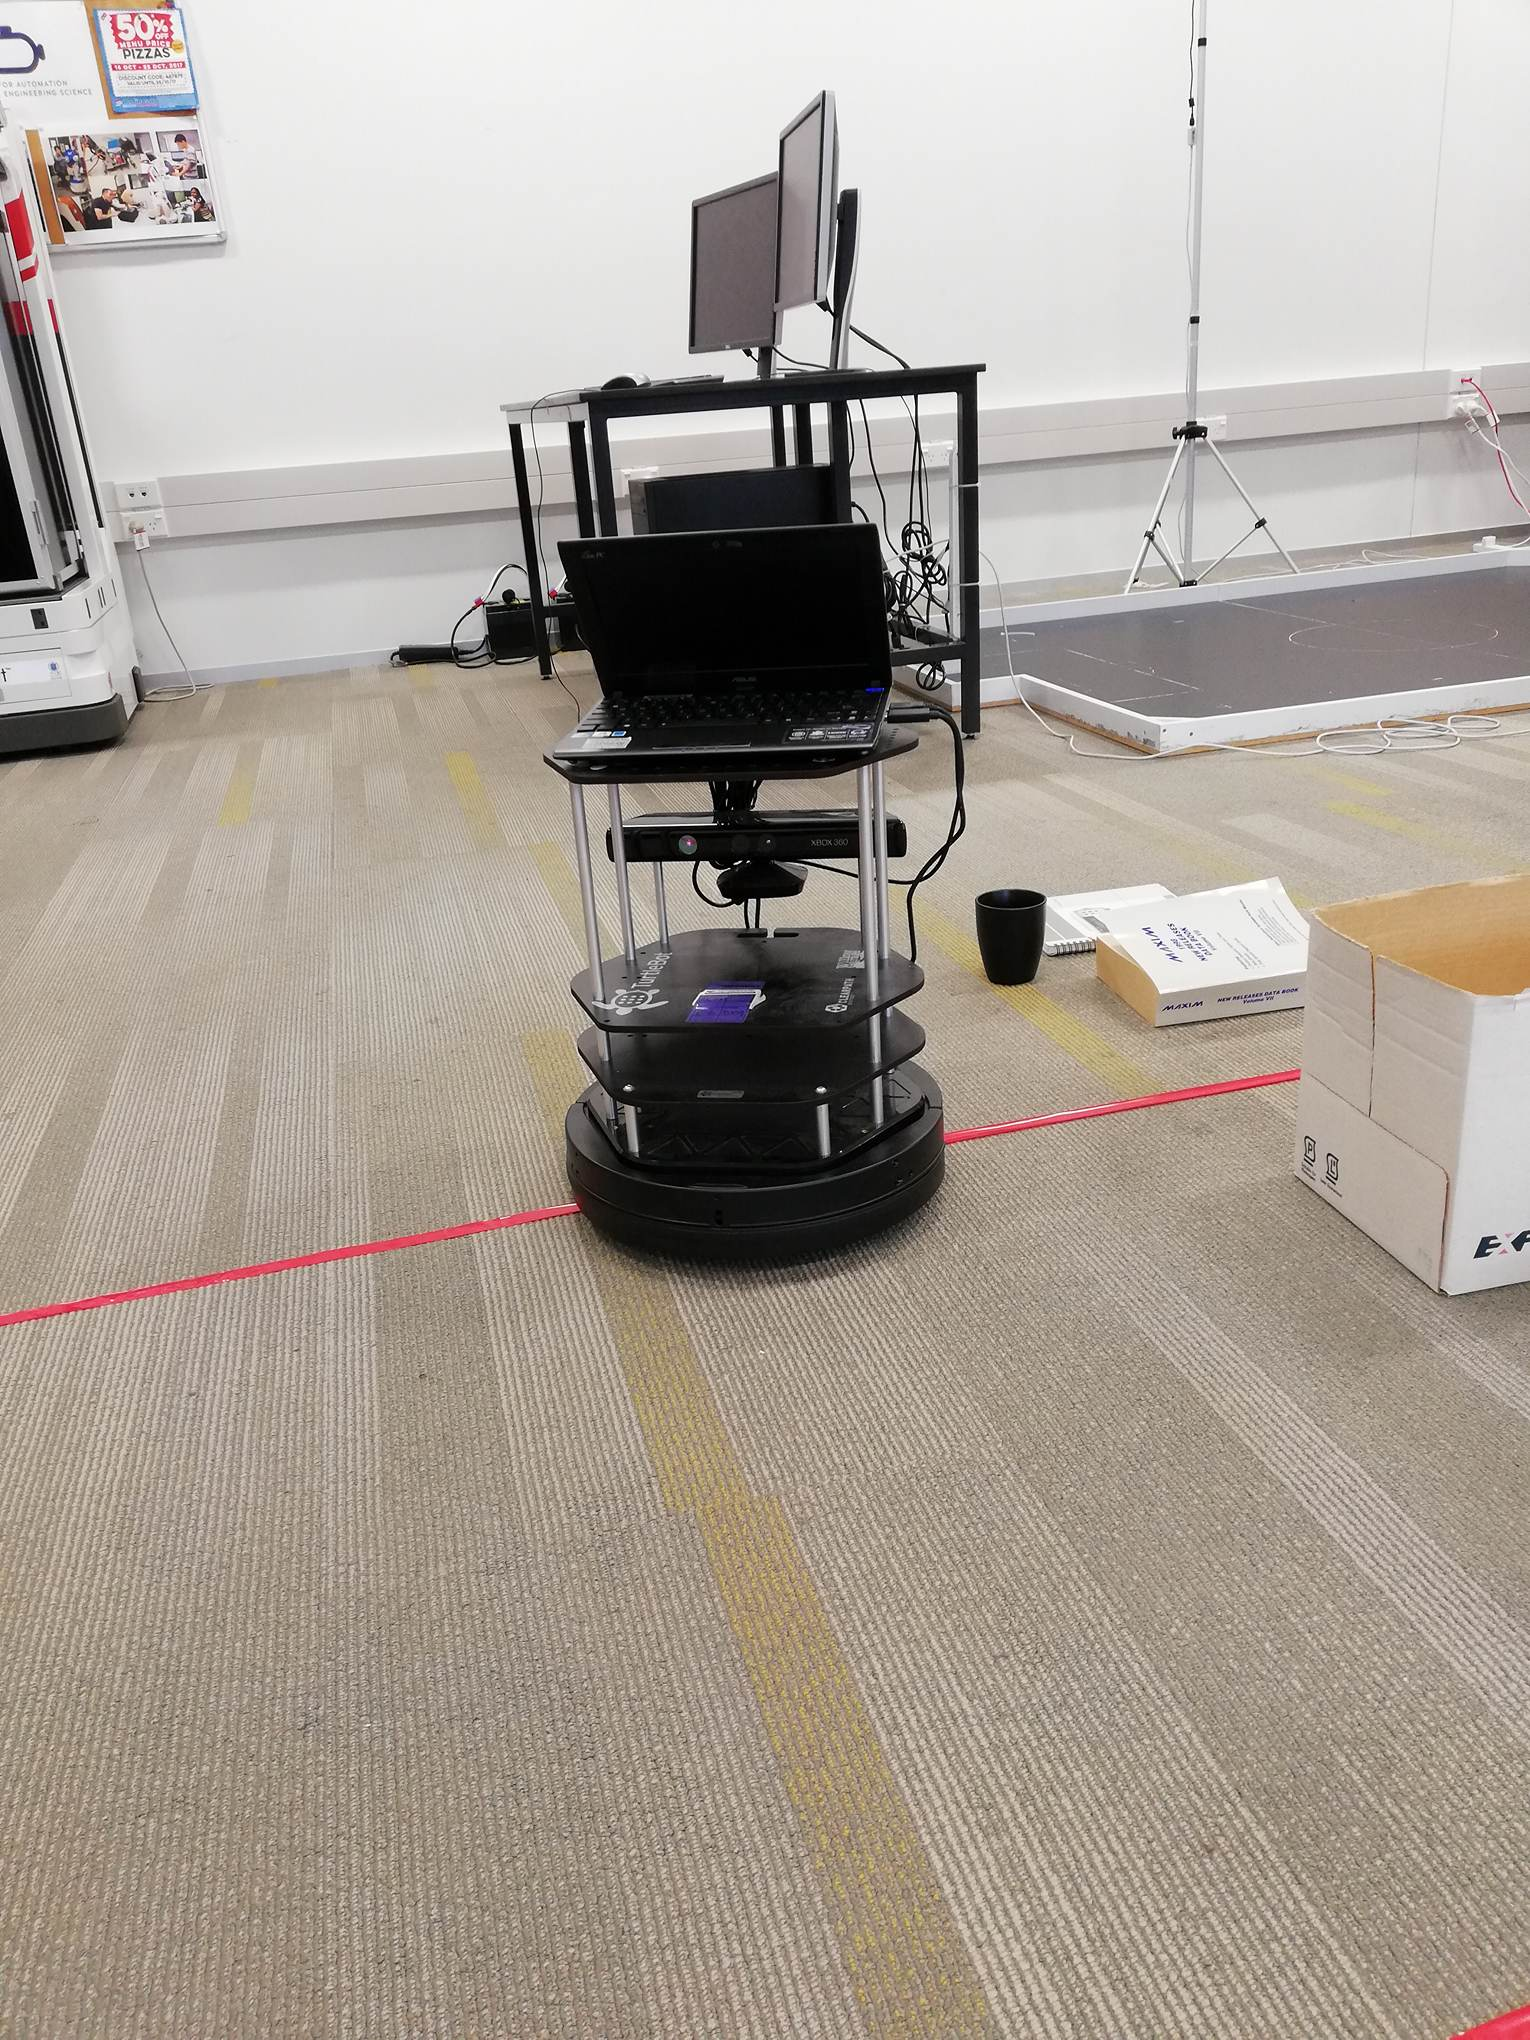
\includegraphics[width=0.31\textwidth]{Images/turtlebot1} \hspace{1em}
%    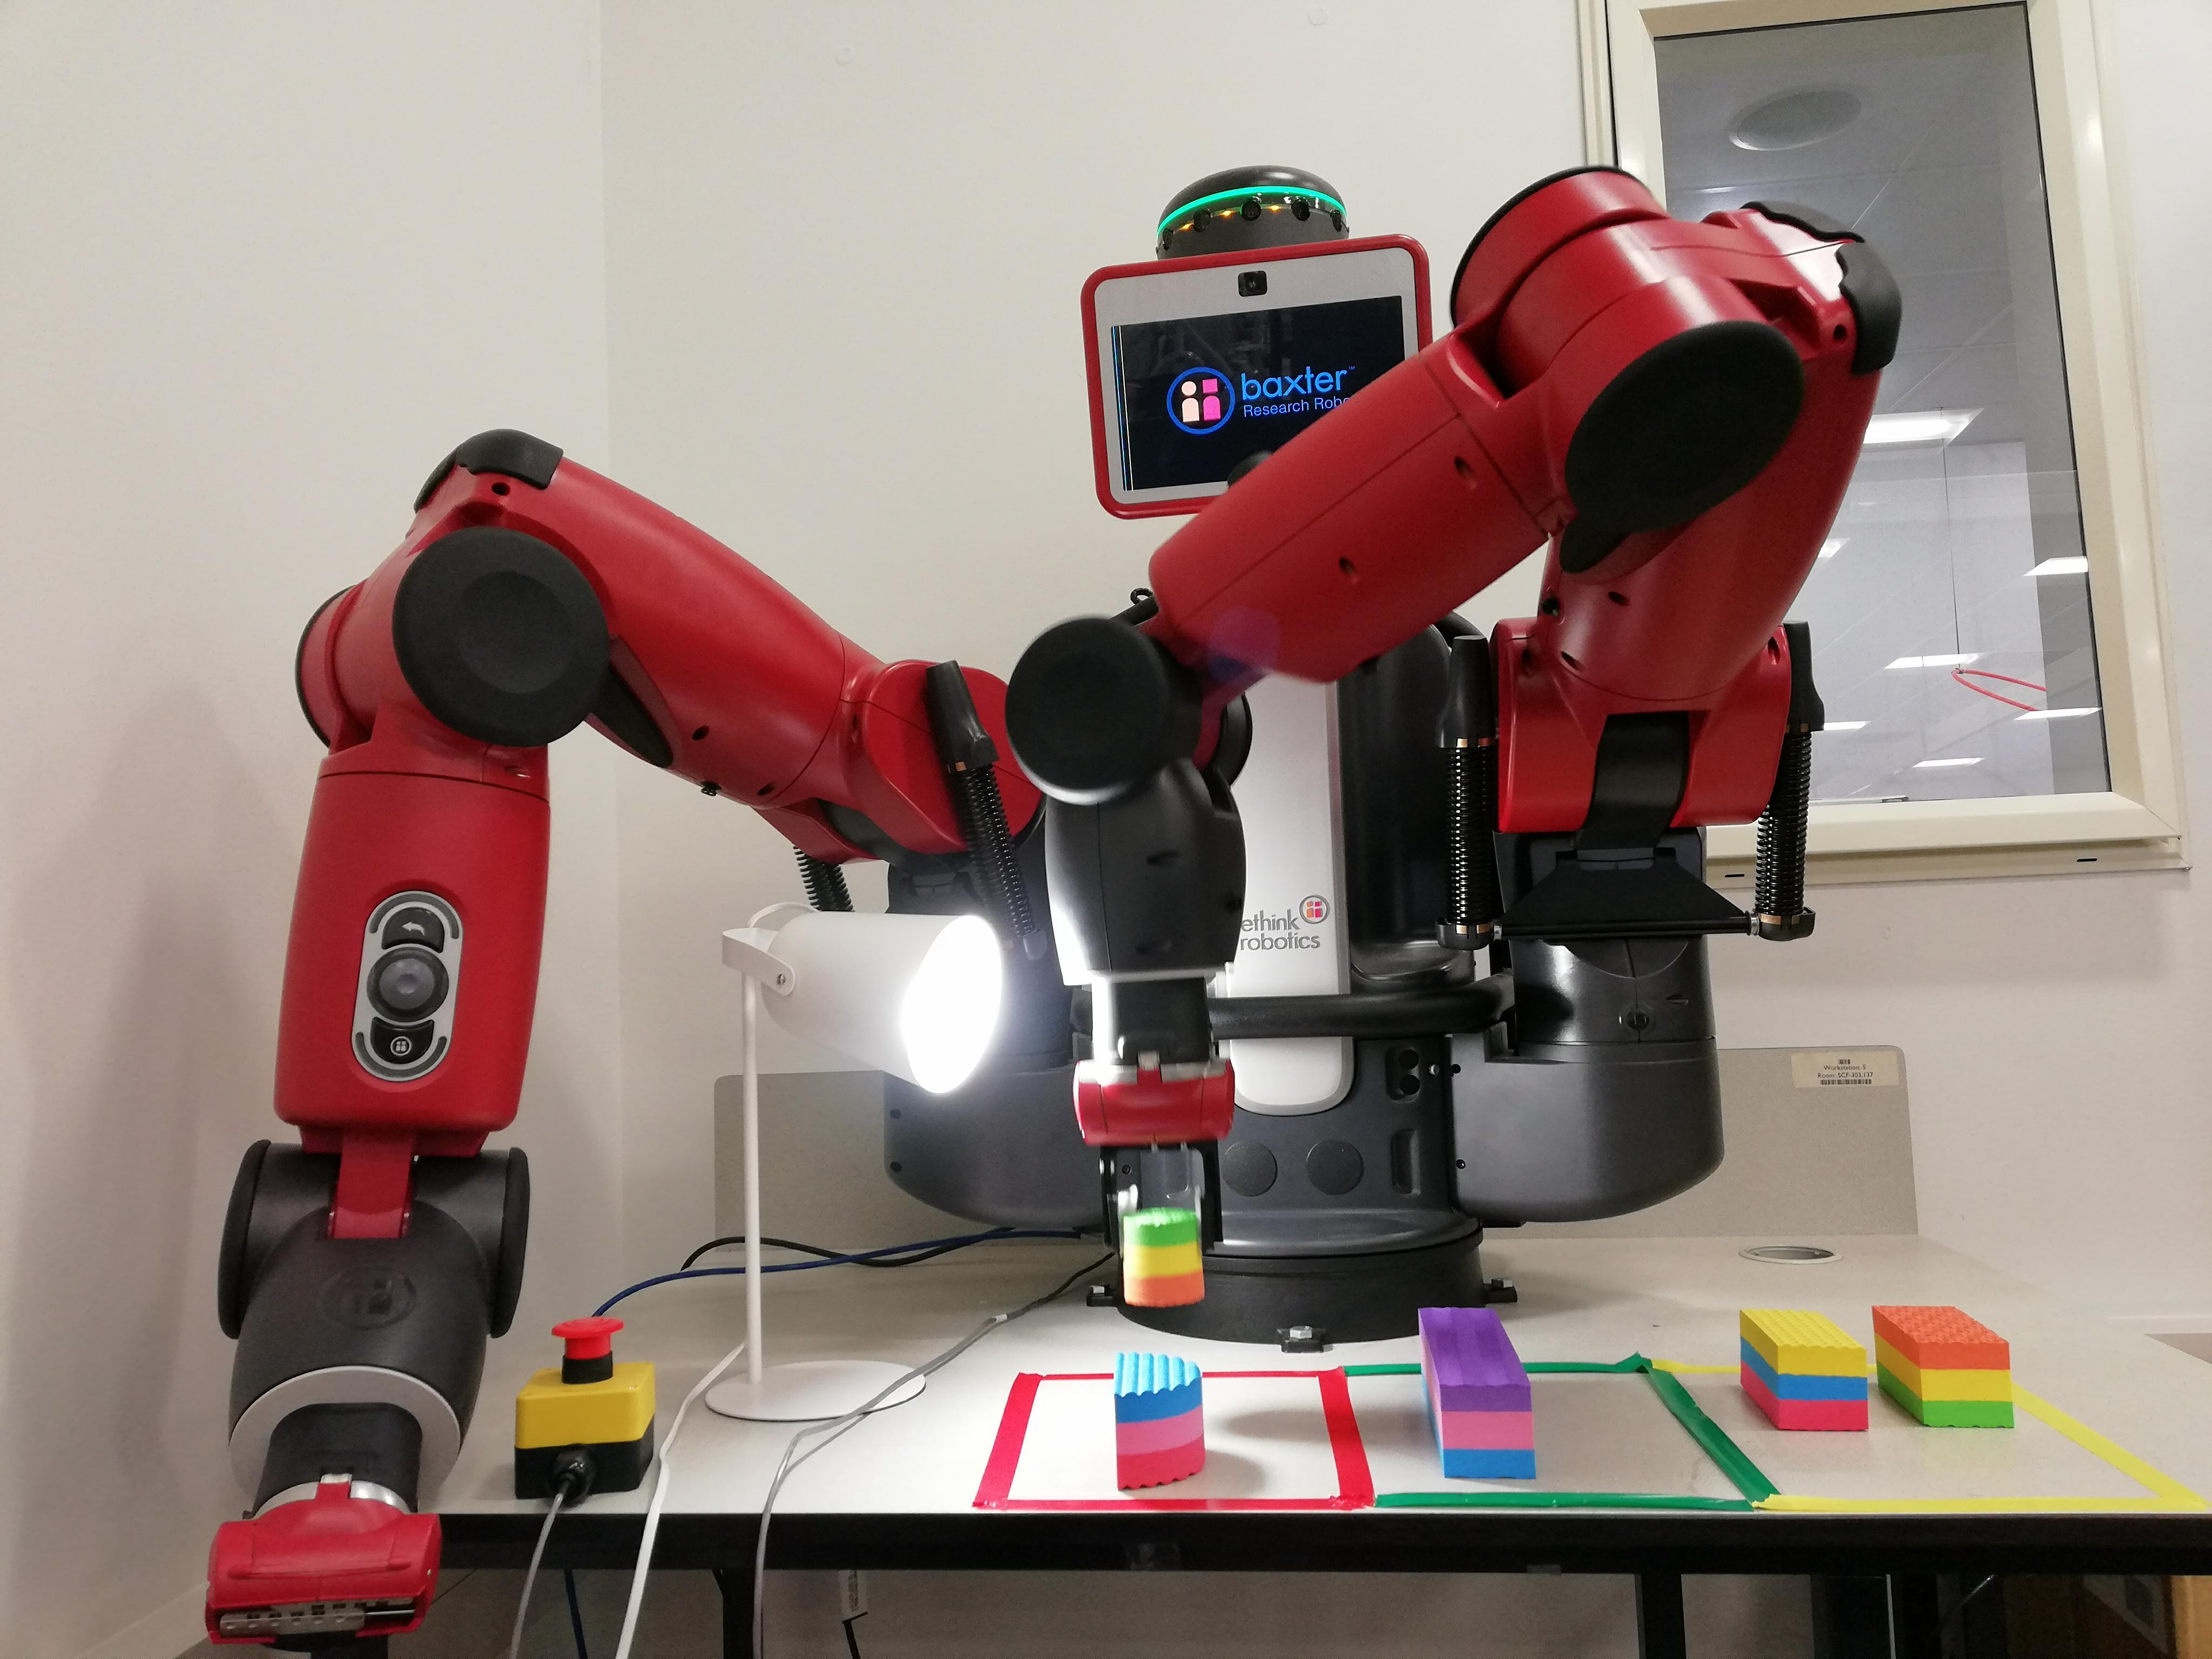
\includegraphics[width=0.50\textwidth]{Images/baxter1}
  \end{center}
  \begin{itemize}
  \item Robot \textcolor{red}{assistant} moving objects to specific
    places.
  \item \textcolor{red}{Sorts}: $robot$, $place$, $object$, $entity$,
    $book$ etc; hierarchical arrangement.

  \item Instances, e.g., \textcolor{red}{place} = $\{of\!\!fice, kitchen,
    library\}$ or $\{red\_area, green\_area, yellow\_area\}$ for tabletop manipulatior.
  \end{itemize}
\end{frame}








\begin{frame}
\frametitle{Illustrative Domain: Robot Moving Objects}

Let us assume that the robot is in the $kitchen$ and its goal is to put the two books in the $library$.
  \begin{center}
    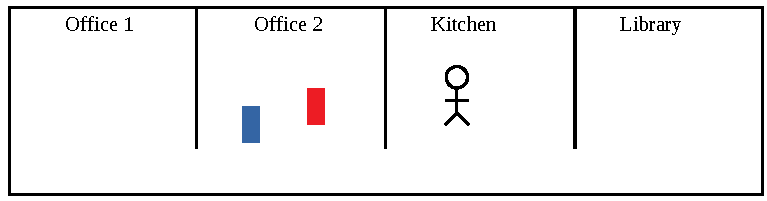
\includegraphics[height=3em]{Images/fourrooms2}\hspace{2em} 
  \end{center}

In traditional planning the robot would:

    \begin{itemize}
    \item Create a plan as a sequence of actions, taking into consideration current beliefs and goal.
    \item Execute the actions of the sequence until one action does not have the expected output.
    \item Replan if necessary.

    \end{itemize}

\end{frame}




\begin{frame}
\frametitle{Illustrative Domain: Robot Moving Objects}
  \begin{center}
    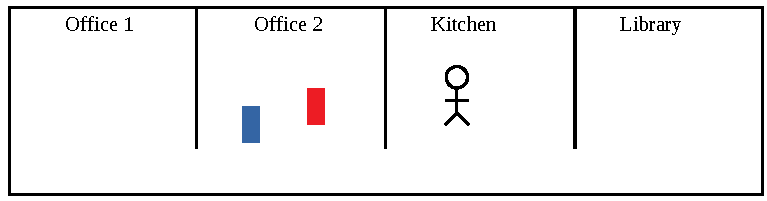
\includegraphics[height=3em]{Images/fourrooms2}\hspace{2em} 
  \end{center}
In a dynamic domain we can have different scenarios:
    \begin{itemize}
    \item While the robot is moving the first book, the second book is moved to the library (\textcolor{red}{unexpected success}).
    \item While to robot is moving the first book, the second book is moved to office\ 1 (\textcolor{red}{not expected to achieve goal - case 1}).
    \item While to robot is moving the first book, the second book is moved to the kitchen (\textcolor{red}{not expected to achieve goal - case 2}).
    \item The robot moves the first book in the library, and when he is putting down the second book, 
the first book is being moved to another room(\textcolor{red}{failure to achieve the goal}).  

     \end{itemize}
\end{frame}


%%%%%%%%%%%%%%%%%%%%%%%%%%%%%%%%%%%%%%%%%%%%%%%%%%%%%%%%%%%%%%%%%%%%%%%%%%%%%%%%
\subsection{Action Language}

\begin{frame}[fragile]{Action Language $AL_d$}
  \begin{itemize}
  \item Formal models of parts of natural language used for describing
    transition diagrams.

    \ \\
  \item Hierarchy of basic \textcolor{red}{sorts},
    \textcolor{red}{statics}, \textcolor{red}{fluents} (basic and
    defined) and \textcolor{red}{actions}.
    
    \ \\
  \item Five types of \textcolor{red}{statements}: 
    \begin{itemize}
    \item Deterministic causal law.
    \item Non-deterministic causal law.
    \item State constraint.
    \item Definition.
    \item Executability condition.
    \end{itemize}
  \end{itemize}
\end{frame}

%     \begin{itemize}
%     \item \textcolor{red}{Deterministic causal laws} $a \
%       \mathbf{causes}\ f(\bar{x})\ = y~\mathbf{if}\ ~body$

%     \item \textcolor{red}{Non-deterministic causal laws} $a \
%       \mathbf{causes}\ f(\bar{x})\ :\ \{Y : p(Y)\} ~\mathbf{if}\
%       ~body$

%     \item \textcolor{red}{State constraint} $f(\bar{x}) = y\
%       ~\mathbf{if}\ ~body$

%     \item \textcolor{red}{Definition} $f(\bar{x})\ ~\mathbf{if}\
%       ~body$

%     \item \textcolor{red}{Executability condition}
%       $\mathbf{impossible}\ a_0,\ldots,a_k \ \mathbf{if}\ ~body$
%    \end{itemize}




%%%%%%%%%%%%%%%%%%%%%%%%%%%%%%%%%%%%%%%%%%%%%%%%%%%%%%%%%%%%%%%%%%%%%%%%%%%%%%%%
%%%%%%%%%%%%%%%%%%%%%%%%%%%%%%%%%%%%%%%%%%%%%%%%%%%%%%%%%%%%%%%%%%%%%%%%%%%%%%%%
\section{Knowledge Representation and Reasoning}

\begin{frame}{Talk Outline}
  \begin{itemize}
    \onslide<0>
  \item  Motivation and overview.
    \ \\
    \ \\
    \ \\
    \onslide<1>
  \item Knowledge representation and reasoning.
    \ \\
    \ \\
    \ \\
    \onslide<0>
  \item Adapted Theory of Intentions.
    \ \\
    \ \\
    \ \\
  \item Experiments and conclusions.
  \end{itemize}
\end{frame}


%%%%%%%%%%%%%%%%%%%%%%%%%%%%%%%%%%%%%%%%%%%%%%%%%%%%%%%%%%%%%%%%%%%%%%%%%%%%%%%%
\subsection{Coarse-Resolution Representation}

\begin{frame}{Logician's System Description}
  \begin{itemize}
  \item Collection of statements of $AL_d$ forms
    \textcolor{red}{system description} $\mathcal{D}_H$, includes
    \textcolor{red}{sorted signature} $\Sigma_H$ and axioms.
    \ \\
    \ \\
  \item \textcolor{red}{Statics}: $next\_to(kitchen, library)$.
    \ \\
    \ \\
  \item \textcolor{red}{Fluents}:\ \\
    $loc : robot \rightarrow place$\ \\
    $in\_hand : robot \times book \rightarrow boolean$
    \ \\
    \ \\
  \item \textcolor{red}{Actions}:\ \\
    $move(robot, place)$\ \\
    $pickup(robot, book)$ 
  \end{itemize}
\end{frame}


 \begin{frame}\frametitle{Logician's System Description}
   \begin{itemize}
   \item \textcolor{red}{Causal laws:}
     \vspace*{-1em}
     {\small
     \begin{align*}
       &move(rob_1, Pl)~~\mathbf{causes}~~loc(rob_1) = Pl \\
       &pickup(rob_1, B)~~\mathbf{causes}~~in\_hand(rob_1, B) %\\ 
     \end{align*}}%
   \ \\

   \item \textcolor{red}{State constraints:}
     \vspace*{-0.5em}
     {\small
     \begin{align*}
       &loc(B) = Pl~~\mathbf{if}~~loc(rob_1) = Pl,~~in\_hand(rob_1, B) \\
       &loc(Th) \not= Pl_1~~\mathbf{if}~~loc(Th) = Pl_2,~Pl_1\neq Pl_2 
     \end{align*}} %
   \ \\

   \item \textcolor{red}{Executability conditions:} 
     \vspace*{-0.5em}
     {\small
     \begin{align*}
       &\mathbf{impossible}~~pickup(rob_1, O)~~\mathbf{if}~~loc(rob_1) \neq ~loc(O) \\
       &\mathbf{impossible}~~pickup(rob_1, O1)~~\mathbf{if}~~in\_hand(rob_1, O2)
     \end{align*}}%

   \end{itemize}
 \end{frame}



\begin{frame}{Logician's Reasoning}



\end{frame}





%%%%%%%%%%%%%%%%%%%%%%%%%%%%%%%%%%%%%%%%%%%%%%%%%%%%%%%%%%%%%%%%%%%%%%%%%%%%%%%%
\subsection{Fine-Resolution Representation}

\begin{frame} \frametitle{Refine + Zoom} 
  \begin{itemize}
  \item Examine system description ($\mathcal{D}_H$) at finer
    resolution ($\mathcal{D}_L$).

  \item Inherit knowledge; add \textcolor{red}{knowledge} fluents and
    actions.


  \item Automatically \textcolor{red}{zoom} to $\mathcal{D}_{LR}(T)$
    relevant to $T=\langle \sigma_1, a^H, \sigma_2\rangle$.

  \item \textcolor{red}{Formal relationships} between descriptions.
  \end{itemize}


\end{frame}



%%%%%%%%%%%%%%%%%%%%%%%%%%%%%%%%%%%%%%%%%%%%%%%%%%%%%%%%%%%%%%%%%%%%%%%%%%%%%%%%
\subsection{Probabilistic Reasoning}

\begin{frame} \frametitle{POMDP Construction}


  \begin{itemize}
  \item $\mathcal{D}_{LR}(T)$ and statistics to construct
    \textcolor{red}{Partially Observable Markov Decision Process}
    (POMDP) tuple $\langle S^L, A^L, Z^L, T^L, O^L, R^L \rangle$.

%     \ \\
%   \item \textcolor{red}{Belief states:} probability distributions over
%     physical states. $B_t = [0.1, 0.8, 0.05, 0.05]$.

%     \ \\
%   \item POMDP \textcolor{red}{solved} to obtain
%     \textcolor{red}{policy} $\pi: B_t\to a_{t+1}^L$.

%     \ \\
%   \item Use policy to repeatedly choose actions, obtain observations
%     and update belief state, until goal achieved with high
%     probability.
    
    \ \\
  \item Add observed outcomes to $\mathcal{H}$ to be used by logician.
  \end{itemize}
\end{frame}




%%%%%%%%%%%%%%%%%%%%%%%%%%%%%%%%%%%%%%%%%%%%%%%%%%%%%%%%%%%%%%%%%%%%%%%%%%%%%%%%
%%%%%%%%%%%%%%%%%%%%%%%%%%%%%%%%%%%%%%%%%%%%%%%%%%%%%%%%%%%%%%%%%%%%%%%%%%%%%%%%
\section{Relational Reinforcement Learning}

\begin{frame}{Talk Outline}
  \begin{itemize}
    \onslide<0>
  \item  Motivation and overview.
    \ \\
    \ \\
    \ \\
  \item Knowledge representation and reasoning.
    \ \\
    \ \\
    \ \\
    \onslide<1>
  \item Adapted Theory of Intentions.
    \ \\
    \ \\
    \ \\
    \onslide<0>
  \item Experiments and conclusions.
  \end{itemize}
\end{frame}


%%%%%%%%%%%%%%%%%%%%%%%%%%%%%%%%%%%%%%%%%%%%%%%%%%%%%%%%%%%%%%%%%%%%%%%%%%%%%%%%
\subsection{Adapted Theory of Intentions}

\begin{frame}\frametitle{Adapted Theory of Intentions}

\end{frame}








%%%%%%%%%%%%%%%%%%%%%%%%%%%%%%%%%%%%%%%%%%%%%%%%%%%%%%%%%%%%%%%%%%%%%%%%%%%%%%%%
%%%%%%%%%%%%%%%%%%%%%%%%%%%%%%%%%%%%%%%%%%%%%%%%%%%%%%%%%%%%%%%%%%%%%%%%%%%%%%%%
\section{Experimental Results and Conclusions}

\begin{frame}{Talk Outline}
  \begin{itemize}
    \onslide<0>
  \item  Motivation and overview.
    \ \\
    \ \\
    \ \\
  \item Knowledge representation and reasoning.
    \ \\
    \ \\
    \ \\
  \item Adapted Theory of Intentions.
    \ \\
    \ \\
    \ \\
    \onslide<1>
  \item Experiments and conclusions.
  \end{itemize}
\end{frame}


%%%%%%%%%%%%%%%%%%%%%%%%%%%%%%%%%%%%%%%%%%%%%%%%%%%%%%%%%%%%%%%%%%%%%%%%%%%%%%%%



%%%%%%%%%%%%%%%%%%%%%%%%%%%%%%%%%%%%%%%%%%%%%%%%%%%%%%%%%%%%%%%%%%%%%%%%%%%%%%%%
\subsection{Experimental Results}

\begin{frame}{Experimental Results: Sepeed and accuracy}

\end{frame}




\begin{frame}{Advantages of Methodology}

\end{frame}



%%%%%%%%%%%%%%%%%%%%%%%%%%%%%%%%%%%%%%%%%%%%%%%%%%%%%%%%%%%%%%%%%%%%%%%%%%%%%%%%
\subsection{Conclusions}

\begin{frame}{Conclusions + Future Work}\small
  \begin{itemize}
    \item \textbf{\underline{Conclusions:}}


    \ \\
  \item \textbf{\underline{Future Work:}}
  \end{itemize}
\end{frame}




%%%%%%%%%%%%%%%%%%%%%%%%%%%%%%%%%%%%%%%%%%%%%%%%%%%%%%%%%%%%%%%%%%%%
%%%%%%%%%%%%%%%%%%%%%%%%%%%%%%%%%%%%%%%%%%%%%%%%%%%%%%%%%%%%%%%%%%%%
\begin{frame}{}
\begin{center}\Large
  That's all folks! 
\end{center}
\end{frame}


%%%%%%%%%%%%%%%%%%%%%%%%%%%%%%%%%%%%%%%%%%%%%%%%%%%%%%%%%%%%%%%%%%%%%%%%%%%%%%%%
%%%%%%%%%%%%%%%%%%%%%%%%%%%%%%%%%%%%%%%%%%%%%%%%%%%%%%%%%%%%%%%%%%%%%%%%%%%%%%%%


\end{document}

%%%%%%%%%%%%%%%%%%%%%%%%%%%%%%%%%%%%%%%%%%%%%%%%%%%%%%%%%%%%%%%%%%%%%%%%%%%%%%%%
%%%%%%%%%%%%%%%%%%%%%%%%%%%%%%%%%%%%%%%%%%%%%%%%%%%%%%%%%%%%%%%%%%%%%%%%%%%%%%%%
